\documentclass{csfourzero}

\title{Latin Authorship Attribution}
\author{Rufus Behr}
\date{\today}
% A useful package to support on-line references
\usepackage{url}
\usepackage{hyperref}
\usepackage{natbib}

\bibliographystyle{plain}
\abstract{
Due to the unique challenges presented by low-resource languages compared to their high resource counterparts, common tasks concerning the style of low-resource language text may require less straightforward approaches. To explore the validity of this claim, this paper investigates authorship attribution, also known as author classification, a common stylometric-based task, in a low-resource language setting --- namely, Latin. In doing so, it sheds light on potential useful features for subsequent stylometric tasks for Latin.
\footnote{Code and data available here: \href{https://github.com/SufurElite/LatinAuthorshipAttribution}{https://github.com/SufurElite/LatinAuthorshipAttribution}}}


\begin{document}
\maketitle


\section{Introduction}
\label{sec:intro}
From analysing Shakespeare to plagiarism-detection, stylometry, the study of style in language, and, in particular, authorship attribution is an active area of research in Natural Language Processing \cite{inproceedings}, but there are unique challenges to conducting analysis in a low-resource language setting. A language is identified as low-resource for its data scarcity or for generally having been studied less than their high-resource counterparts as defined by Magueresse et al. \cite{https://doi.org/10.48550/arxiv.2006.07264}.  Moreover, there are further complications as style can be difficult to recognise computationally given its inherent qualitative nature, and, although for most high-resource languages this can be overcome by applying straightforward techniques with vast amounts of data, that is not always feasible for low-resource languages and may require more creative solutions \cite{inproceedings}. 

Stylometry, however, predates the existence of computational linguistics. For example, in the early 20$^{\text{th}}$ century, prospective Classics students for Oxford University were required to write text in the style of particular authors (Cicero, Catullus, etc.). An overarching aim for this paper was to provide a foundation for further work to build upon in order to pass this Oxford entrance exam computationally; more explicitly, the future work will aim to generate author-styled text akin to research done by Tikhonov and Yamshchikov, which employed an LSTM architecture with phonetic and semantic embeddings to generate English and Russian stylized poetry \cite{Tikhonov_2018}, but for Latin, a comparatively low-resource language. 

Thus, the research interest in this paper is to provide this foundation by performing authorship attribution, classifying texts by their authors. If it is possible to distinguish authors based solely on features extracted from their work, it lends credence to the idea that the style of these authors is implicit in their work, which is a prerequisite for generating text in their style. Furthermore, this paper will shed light precisely on the features that will be best suited for fine-tuning the authors’ styles for text generation. 

\section{Background and Related Work}
\label{sec:lit}
There has been prior work on clustering and determining the authors of Latin texts; in these works, the authors investigate the effectiveness of applying clustering techniques on documents encoded by Latin word embeddings. In a paper by Burns et al., they train word2vec word encodings on a large Latin corpus to perform intertextual profiling (even finding semantically similar passages - not necessarily verbatim equivalents) and another set of embeddings on a small authorial corpus to show that it captures the writing style by replicating a prior intertextual study of that author \cite{burns-etal-2021-profiling}. They suggested for future work that a similar study can be done but with contextual word embeddings, such as Latin-BERT \cite{https://doi.org/10.48550/arxiv.2009.10053}, rather than static ones, and this is precisely what Bernardo et al. undertake. In their work, they encode the different documents using Latin-BERT, calculate the cosine similarity between authors’ texts, and perform a k-means clustering algorithm on the texts to identify the respective similarities with an accuracy of 91$\%$ \cite{https://doi.org/10.48550/arxiv.2109.00601}. However, they restrict themselves by using just one Latin dataset and they only present the results of using Latin-BERT rather than comparing the results of Latin-BERT with word2vec. Another potential area for improvement would be to use Vec2GC, a clustering algorithm developed by Rao and Chakraborty, which was designed particularly for clustering text representations \cite{https://doi.org/10.48550/arxiv.2104.09439} and was shown to have better performance over k-medoids (a similar algorithm to k-means). 

Unlike word embeddings for high-resource languages, Sprugnoli et al. caution that Latin word embeddings may face challenges by being comparatively low-resource and instead created lemma embeddings for Latin \cite{Sprugnoli2020BuildingAC}, which refers to collating the same word regardless of its contextually dependent ending. The word2vec approach by Burns et al. circumvents this issue by making use of the Classical Language Toolkit \cite{johnson-etal-2021-classical} to lemmatize words prior to training.

In the work detailed above, they use embeddings to show the semantic similarity between documents, which can then be used for different tasks including authorship attribution. Kim et al.’s paper on literary style classification, identifies further features that might help with text classification including basic (word frequency statistics), syntactic (part of speech tagging), semantic (synonyms of words), and manual features (creating rules from human observations about the text) \cite{Kim2011LiterarySC}. The improved performance from the inclusion of these features aligns with the thoughts shared by Lagutina et al. in their survey on stylometric text features. They explain that, although a lot of the best results come from straightforward features, it's because of how easily derivable (for a computer) the features are compared to classical linguistic features, which might improve the results but are harder to automate comparatively \cite{inproceedings}. Lagutina et al. in a subsequent paper then presented novel algorithms to automatically extract such features --- namely, the use of repetitive literary devices (anaphora, polysyndeton, etc.), the frequency of which they plotted over time to show changes in usage over history \cite{lagutina2020automatic}. 

Rhythmic features are also the subject of interest in a paper by Corbara et al. where the authors explore the efficacy of syllabic quantity patterns - effectively, rhythm - for Latin authorship attribution. They investigate the use of these features by having base features (common syntactic features found in authorship attribution) and introducing new features (derived from the scansion, the metrical patterns, of the text) \cite{SyllabicQuantity}. They purport having improved accuracy by the inclusion of these models across different datasets, but they do not make use of models that provide more interpretability, which would help explain the importance of these features for classification. 

Lastly, authorship attribution has been the primary focus of the papers detailed to encapsulate the notion of style within text. In Cook’s \textit{What would Cicero write?}, he trains a language model to predict a missing word that is intentionally removed from sentences in Cicero’s work \cite{Cook_2021}. Whilst this is closer to the natural language generation proposed as future work in Section \ref{sec:intro}, an argument can be made that this also encapsulates style and could be interesting to see the effects of predicting on the same masked sentence after training under different authors' texts.

\section{Research Question}
\label{sec:rq}

Before being able to tackle the larger task of generating author-styled text in Latin, it is prudent to first discern whether the styles of these authors are distinguishable, and, if so, it is worth investigating what most distinguishes their styles. Having established the idea of stylometry and then having reviewed computational methods to perform authorship attribution, the research questions follow naturally:
\begin{enumerate}
    \item Are the styles of the Latin texts distinct enough to accurately classify by author semantically? Additionally, how do the varying word embeddings compare in encoding the semantic relation between documents to perform this task?
    \item Are syntactic and rhythmic features in Latin texts enough to classify the author? Is it possible to identify the most important stylometric features for authorship attribution? If so, what are they?
\end{enumerate}
The expected answer to the first question was yes, given the success of the approaches detailed, and, in the follow-up question, Latin-BERT was expected to outperform the other embeddings on account of its contextuality. With regards to the second question, given the results of Corbara et al. \cite{SyllabicQuantity}, it was expected that the syntactic and rhythmic features would be sufficient to classify the authors. Furthermore, through a combination of testing with and without particular features, it was expected to be able to calculate the potency of the feature from its improved, stagnant, or lessened accuracy. If that was the case, then the rhythmic features, using the same feature extraction as in Corbara et al. \cite{SyllabicQuantity}, were expected to improve the accuracy of the model. 

Before being able to start this investigation, there was some minor preprocessing work required. For all the tasks it was useful to have a unified Latin corpus spanning multiple datasets. The main obstacle in creating a unified corpus was to use the differently formatted datasets without including multiple entries of the same text, as some of the texts are present across the corpora. Storing only distinct texts, however, can be accomplished by parsing the different formats and then, once all the texts have been added, performing a longest common substring on the list of words to identify texts with an overlap above an arbitrary similarity threshold (e.g. if one document shares over 70$\%$ of its text with another, then one of the documents should be removed). Once the corpus was created and minor exploratory data analysis was performed (e.g. finding out the distribution of text across authors, statistics about the authors' texts, etc.), experimentation to answer the research questions began. The next objective was to replicate the paper by Bernardo et al. \cite{https://doi.org/10.48550/arxiv.2109.00601}. And, the final objective was to develop a separate classification method like the one in Corbara et al. \cite{SyllabicQuantity} that compared the base syntactic features and derived rhythmic features to perform authorship attribution, but, additionally, to train a Random Forest Classifier to have better interpretability about which features were most useful, whence future work concerning natural language generation can build upon in a more informed manner. 


\section{Experimental Design}
\label{sec:exp}

Recalling the research questions and hypotheses from above, hereupon, when discussing the different questions, we will divide them into Semantic and Stylometric subsections respectively. For both sections, the text for the experimentation was selected from the corpus by identifying the 25 authors with the most extant text. 

\subsection{Semantic Experiments}
The aim for the semantic experiments is to accurately classify the documents by their respective authors using pre-trained semantic word embeddings --- namely, Latin BERT \cite{https://doi.org/10.48550/arxiv.2009.10053} and The Classical Language Toolkit's word2vec embeddigns \cite{johnson-etal-2021-classical}.
The text first will be preprocessed by including only unicode characters, making all the text lowercase, and stripping punctuation. Afterwards, the same text documents will be encoded by the different word embeddings, where each document will be represented by the average of the word embeddings across documents, and then two means of classification will be done: supervised and unsupervised. For supervised, the encoded documents will be the input to a support vector machine with the authors as the output, and, for the unsupervised, as in Bernardo et al. \cite{https://doi.org/10.48550/arxiv.2109.00601}, a k-means clustering algorithm will fit on the data with the number of clusters, k, being equal to the number of authors. The correctness of the clustering algorithm, as the cluster labels will be randomly determined and therefore not correspond to the author labels, will be evaluated by using a rand score, which finds the most correlated permutations of the predicted clusters labels and the correct author labels and returns the percentage. The accuracy and the rand score will answer the first part of the Semantic research question --- whether the styles of the text are distinct enough semantically to classify the author, and so, if these metrics are greater than by random selection, then the proposed hypothesis holds.

In order to determine the second part of the research question, identifying which word embeddings perform better for this task, it is first worth noting that the models will have been trained on the same hyperparameters with the same training and testing examples. Thus, to determine if one embedding performs better for the task the predicted results from the first part of the experiment will be used to create a McNemar contingency table and then the McNemar test  --- with a null hypothesis that the models are not different --- will be applied, validating if the predicted samples are significantly different with a p-value of $0.05$.

\subsection{Stylometric Experiment}
The text for the stylometric experiments will be preprocessed in a similar manner to the semantic experiment, but there is the additional inclusion of the scansion of the texts. The raw texts, along with the scanned texts, are then passed into the feature extractor used in Corbara et al.\cite{SyllabicQuantity}, which extracts the following features
\begin{itemize}
    \item Base Features:
    \begin{itemize}
        \item Frequency of function words --- i.e. grammatically functional words rather than lexically rich (prepositions, conjunctions, etc.)
        \item Frequency of words of length, spanning 1 character to 25 characters
        \item Frequency of sentence length, spanning 1 word to 100 words
    \end{itemize}
    \item Metre-related Features:
    \begin{itemize}
        \item Distorted View: Single Asterisks (DVSA), where every non-functional word is replaced by an asterisk
        \item Distorted View: Multiple Asterisks (DVMA), where every character in a non-functional word is replaced by an asterisk
        \item Syllabic Quantity (SQ) N-Grams: n-grams but of the metric patterns (long syllable, short syllable, or short or long syllables) rather than words
    \end{itemize}
\end{itemize}

 To answer the first part of the stylometric research question, a support vector machine and a random forest classifier were trained on all the features to establish if the first stylometric hypothesis is correct --- whether the authors of documents can be determined through these features. 
 
 In order to address the second part of the question, these two classifiers were then trained on just the semantic features and then trained with the inclusion of the rhythmic ones. As above, to see if the inclusion of the rhythmic features provides any significant difference of the predicted sample output, the contingency table is computed and a McNemar test employed. 
 
 Lastly, to further address which features are most important for authorship attribution the individual features of the Random Forest Classifier were inspected, which directly shows their importance in prediction\footnote{Note that the features belong to groups as detailed above - frequency of function words, frequency of word length, etc., so the individual features are grouped for easier readability rather than inspecting and plotting each of the 938 features individually}. 
\section{Results}
\label{sec:results}
As the experiments were divided by semantic and stylometric research questions so too are the reported results.
\subsection{Semantic Results}
Attempting to encode the documents using the BERT word embeddings consistently crashed the code, so unfortunately only CLTK’s word2vec embeddings were used and the second part of the semantic research question was unanswerable. The k-means clustering achieved a rand score of 89$\%$ and the support vector machine achieved an accuracy of 86$\%$, so the models were able to distinguish more than randomly satisfying the first part of the semantic research question, confirming that research hypothesis. The predictions made by the support vector machine on the test set (compared to the ground truth test set) are visualised in Figure \ref{fig:SVM_UMAP}. To create the plot the feature space of the embeddings were mapped down to two dimensions using UMap.
\begin{figure}[hbt!]
    \centering
    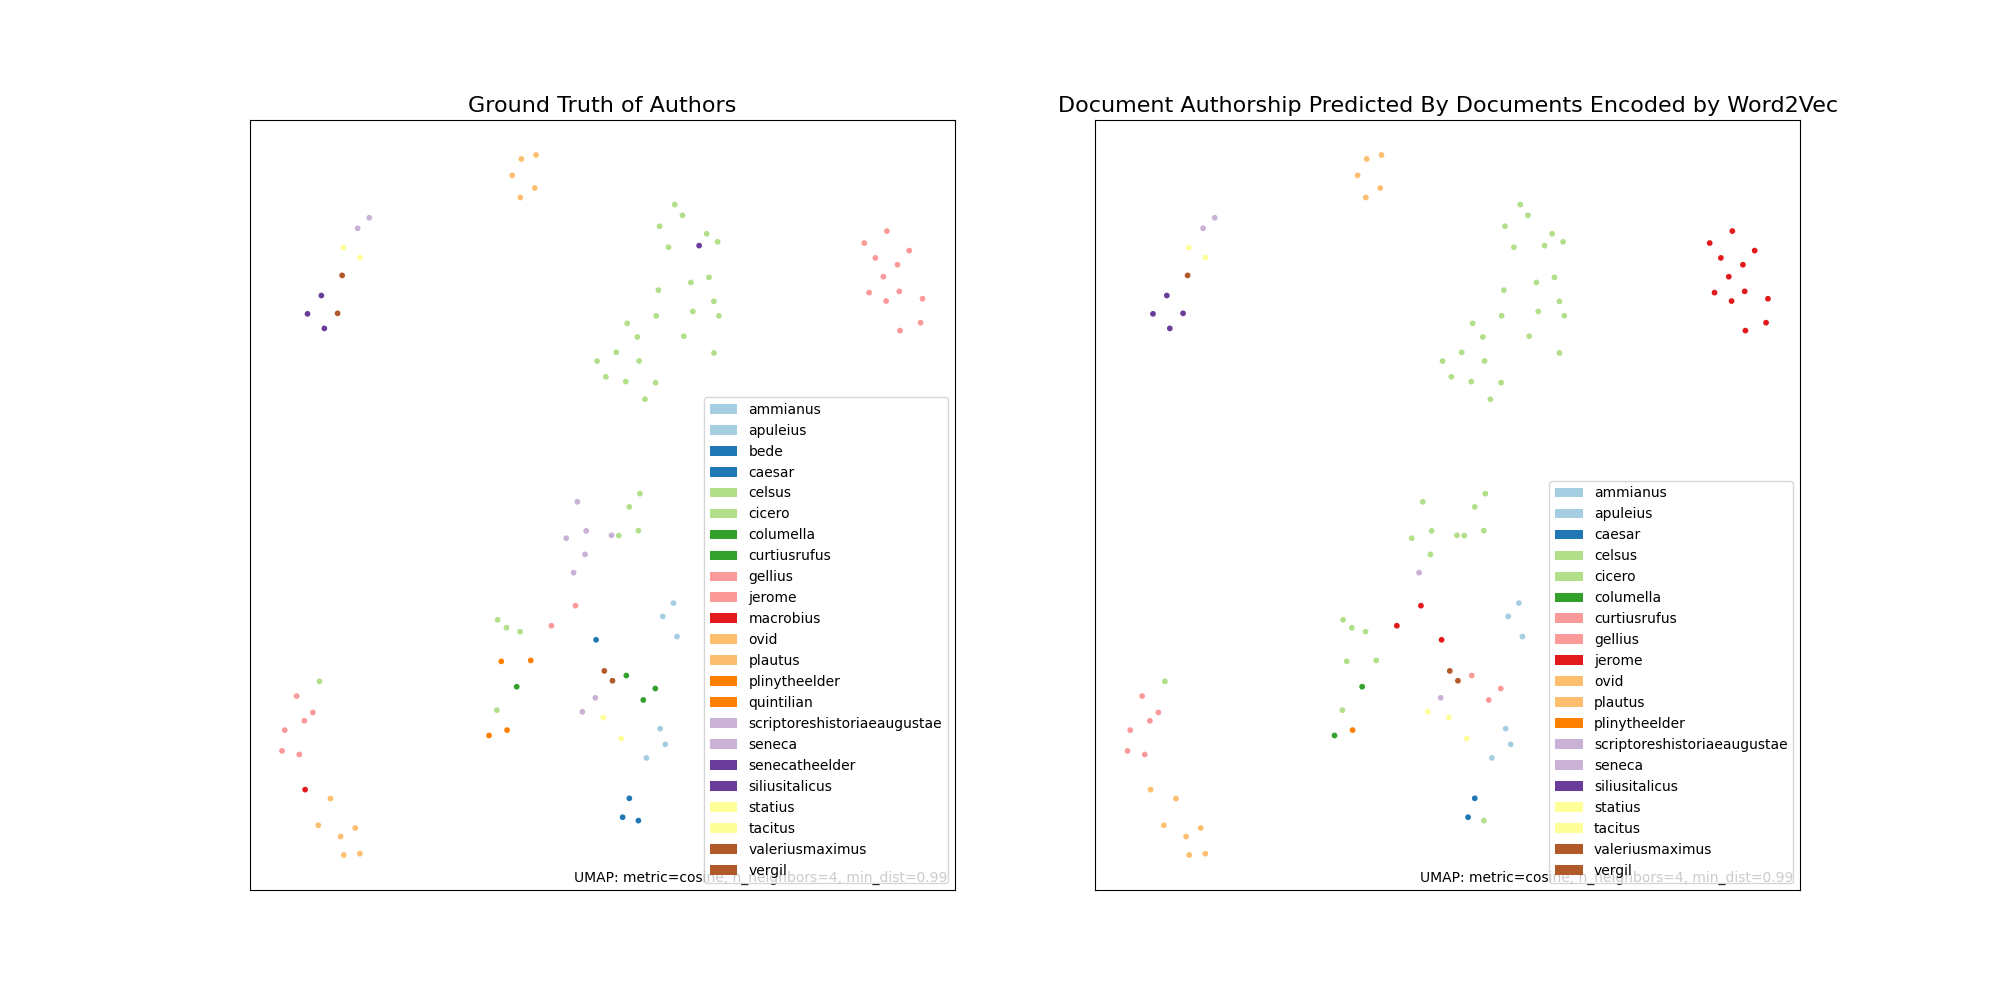
\includegraphics[width=6in]{SVM Documents Predicted on Word 2 Vec.png}
    \caption{Support vector machine predicted on word2vec Embedded Documents (note the colours are not necessarily the same for each author across the plots)}
    \label{fig:SVM_UMAP}
\end{figure}

\subsection{Stylometric Results}
On the data that used both the syntactic and rhythmic features, on the test data the support vector machine achieved an F1 score of 85.6$\%$ and an accuracy of 86.6$\%$ and the Random Forest achieved an accuracy of 82$\%$, so the models were able to classify the authors using these features, confirming that hypothesis. Having established that these features can be used for classification, the next point of interest is the significance of the different features. When testing on just the syntactic features, the models on average had a lower accuracy. In one run, the SVM McNemar table, where we compared the predictions of the same models to determine if there was a statistically significant difference in the predictions using the two datasets, produced the results in Table \ref{tab:McNemarOutlier}.
\begin{center}
\begin{table}[hbt!]
    \centering
    \begin{tabular}{c|c | c}
     & model 2 correct & model 2 incorrect \\ \hline
     model 1 correct & 183 & 15 \\ \hline
    model 1 incorrect & 0 & 26 \\
    \end{tabular} 
    \begin{tabular}{c c}
     $\chi^{2}$: & 13.066666666666666 \\ 
     p-value: & 0.00030059760744045053
    \end{tabular}
    \newline
    
    
    \caption{McNemar Table Outlier where model 1 contains the rhythmic data as well as syntactic and model 2 only contains syntactic}
    \label{tab:McNemarOutlier}
\end{table}

\end{center}
This, however, was deemed to be an anomaly by running k-folds cross validation (where one fold is the test set) and calculating the McNemar table for the model’s test predictions on each fold. This resulted with a much larger average p-value (~.5-.6) and a minimum p-value of ~.13. Therefore, we accept the null hypothesis that there is no difference between the samples, which would also reject the hypothesis on the rhythmic features being of signficantly more importance.
\begin{figure}[hbt!]
    \centering
    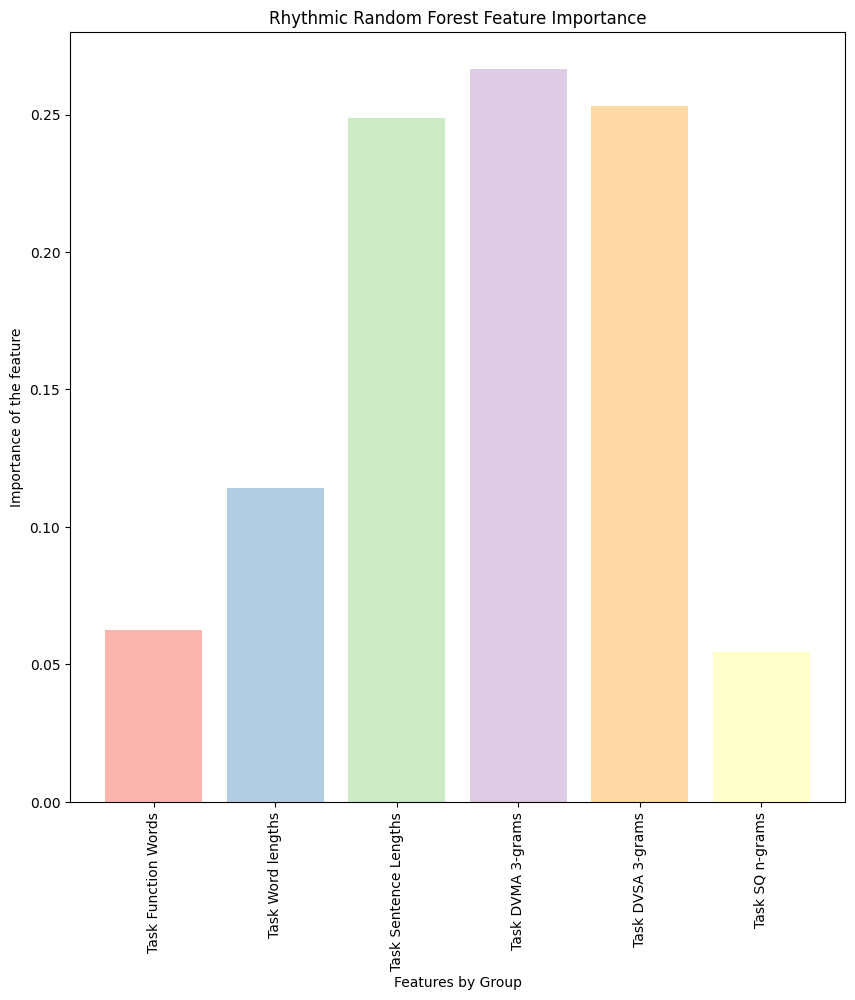
\includegraphics[width=3in]{Rhythmic Random Forest Feature Importance.png}
    \caption{Random Forest Feature Importance}
    \label{fig:RandomForest}
\end{figure}
\newline 
To get a better idea of which features were important, after training the random forest classifier, the feature importances of the classifier were grouped together by their association and then plotted in Figure \ref{fig:RandomForest}. This figure shows that the DVMA and the DVSA features in addition to the sentence length were very important.
\section{Discussion}
\label{sec:discuss}

The results show that Latin authorship attribution is feasible using either semantic, syntactic, or syntactic and rhythmic features to discriminate the authors. It, however, does not show that the inclusion of non-standard features necessarily bolsters the algorithms' performances by a considerable margin, as was initially suspected, but there may be other non-standard features that should have been considered, such as those mentioned in Lagutina et al. \cite{lagutina2020automatic}, which should be investigated. Even though the classifiers didn't significantly improve with the inclusion of other features, when analysing the feature importances of the random forest classifier, the importance of both the DVMA and DVSA features are pronounced. 

Moreover, there are a number of areas where further work can address the potential shortcoming of this paper. Most notably, further experimentation is required for evaluating the difference between using word2vec and Latin BERT for authorship attribution, as that was a question this paper was unable to address. Even though the syllabic quantity feature had the lowest importance, it is possible that the text selected from the corpus was not conducive to being significantly metrically different.
For instance, further experimentation where the text is entirely poetry rather than prose may better utilise the metre of the text. Additionally, it would be interesting to see how a model that incorporates both the semantic features of the text using a word embedding as well as the syntactic and rhythmic features performs comparatively. 



\section{Conclusion \& Future Work}
\label{sec:conc}

I have conducted experiments to determine if it is possible to perform Latin authorship attribution using semantic, syntactic, and syntactic and rhythmic features. Then, I also conducted experiments to determine which features are most efficacious at performing this task. This was all with the aim of developing a foundation for subsequent work on the generation of Latin texts in the style of particular authors. Being able to classify who wrote a particular document implies a recognition of authorial style and the important features for that classification may also prove to be useful in producing text in authorial style.

I have shown through the experiments that Latin authorial style can be identifiable by machine and have provided some initial feature importances, whence to take inspiration for stylistic generation. 

\section{Reflective Analysis}

Whilst there is plenty I would repeat and I thought worked well (e.g. using the Classical Language Toolkit, deriving feature importance from a random forest classifier, etc.), there are a number of things I would change given the chance to start all over. First and foremost, I would likely run the code from google colab or another server with larger memory capacity than my laptop, which would allow for the inclusion of experimenting with Latin BERT more easily. I would also write the unifying Latin corpus code using parallelization as the longest common substring across all of the authors' texts is time-consuming and can be done concurrently. Lastly, I would try to incorporate more rhythmic or non-standard features for analysis.

\newpage
\nocite{*}
\bibliography{myrefs}

\end{document}
